\documentclass{ximera}

\input{../preamble.tex}


\title[Problem 3]{Problem 3}

\begin{document}
\begin{abstract} \end{abstract}
\maketitle


% Extracted from maximumsAndMinimums.tex, problem #3
\begin{problem}
For each point in the interval (a,b)  and identified on the graph below, determine if the function $f$ has a critical point, a local max or min at that point.\\


%	\begin{center}
%	\begin{image}
%	
\includegraphics{figure3_pdf.png}
%	\end{image}
%	\end{center}	

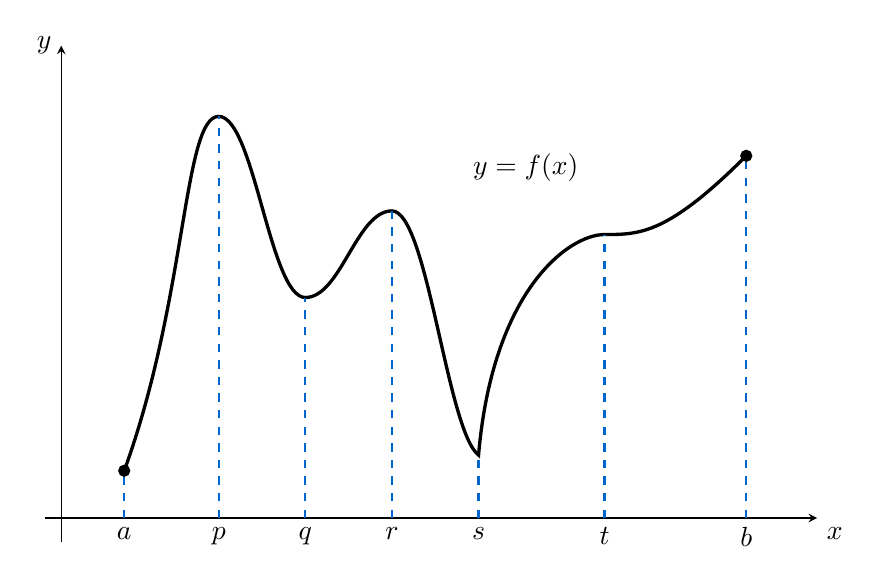
\begin{tikzpicture}[x=1cm,y=1cm,>=stealth]
		%---------------- Colors & styles ----------------
		\definecolor{accent}{RGB}{0,102,204} % blue for vertical guides
		\tikzset{
			func/.style={very thick, black},                 % graph color
			vmark/.style={accent, dashed, line width=0.8pt}, % vertical dashed lines
			endpoint/.style={black, fill=black, draw=black}, % endpoint dots
		}
		
		%---------------- Labeled x-positions ----------------
		\def\xa{0.8}
		\def\xp{2.0}
		\def\xq{3.1}
		\def\xr{4.2}
		\def\xs{5.3}
		\def\xt{6.9}
		\def\xb{8.7}
		
		%---------------- y-values at those x’s ----------------
		% p is the global max; b is high but < p
		\def\ya{0.6}  % a
		\def\yp{5.1}  % p (GLOBAL MAX)
		\def\yq{2.8}  % q (local min)
		\def\yr{3.9}  % r (local max)
		\def\ys{0.8}  % s (local min, sharp corner)
		\def\yt{3.6}  % t (horizontal tangent)
		\def\yb{4.6}  % b (endpoint)
		
		% Horizontal tangent control length at p, q, r, t
		\def\dh{0.45}
	
		
		%---------------- Axes ----------------
		\draw[->] (-0.2,0) -- (9.6,0) node[below right] {$x$};
		\draw[->] (0,-0.3) -- (0,6.0) node[left] {$y$};
		
		%---------------- Graph y = f(x) ----------------
		% Smooth at p, q, r, t (horizontal tangents), corner at s,
		% concave down on (s,t), concave up on (t,b).
		\draw[func]
		% a -> p : increasing; arrive p horizontal
		(\xa,\ya)
		.. controls (\xa+0.80,\ya+2.20) and (\xp-\dh,\yp) .. (\xp,\yp)
		% p -> q : decreasing; horizontal at p and q
		.. controls (\xp+\dh,\yp) and (\xq-\dh,\yq) .. (\xq,\yq)
		% q -> r : increasing; horizontal at q and r (C^1 smooth at r)
		.. controls (\xq+\dh,\yq) and (\xr-\dh,\yr) .. (\xr,\yr)
		% r -> s : decreasing; leave r horizontal (C^1), arrive at s (corner)
		.. controls (\xr+\dh,\yr) and (\xs-0.40,\ys+0.30) .. (\xs,\ys)
		% s -> t : increasing, CONCAVE DOWN, arrive t horizontal
		.. controls (\xs+0.18,\ys+2.10) and (\xt-\dh,\yt) .. (\xt,\yt)
		% t -> b : increasing, CONCAVE UP, leave t horizontal
		.. controls (\xt+\dh,\yt) and (\xb-1.00,\yb-1.00) .. (\xb,\yb);
		
		%---------------- Label ----------------
		\node[black] at (5.9,4.45) {$y=f(x)$};
		
		%---------------- Blue dashed verticals that stop at the graph ----------------
		% Direct to the known points on the curve (no intersections needed)
		\draw[vmark] (\xa,0) -- (\xa,\ya);  % a
		\draw[vmark] (\xp,0) -- (\xp,\yp);  % p
		\draw[vmark] (\xq,0) -- (\xq,\yq);  % q
		\draw[vmark] (\xr,0) -- (\xr,\yr);  % r
		\draw[vmark] (\xs,0) -- (\xs,\ys);  % s
		\draw[vmark] (\xt,0) -- (\xt,\yt);  % t
		\draw[vmark] (\xb,0) -- (\xb,\yb);  % b
		
		%---------------- x-axis labels ----------------
		\node[below] at (\xa,0) {$a$};
		\node[below] at (\xp,0) {$p$};
		\node[below] at (\xq,0) {$q$};
		\node[below] at (\xr,0) {$r$};
		\node[below] at (\xs,0) {$s$};
		\node[below] at (\xt,0) {$t$};
		\node[below] at (\xb,0) {$b$};
		
		%---------------- Endpoint dots (same color as graph) ----------------
		\fill[endpoint] (\xa,\ya) circle (2pt);
		\fill[endpoint] (\xb,\yb) circle (2pt);
	\end{tikzpicture}


\begin{explanation}


(p) The function $f$ has a critical point and a local maximum at $x=p$.  

(q) The function $f$ has a critical point and a local minimum at $x=q$.

(r) The function $f$ has a critical point and a local maximum at $x=r$

(s) The derivative of $f$ does not exist at $x=s$ because the function $f$ has a corner at $x=s$.  The function has a critical point and a local minimum at $x=s$.

(t) The function $f$ has a critical point but not a local maximum or minimum at $x=t$.


		\end{explanation}	
		
\end{problem}



\end{document}
